\documentclass[aspectratio=169]{beamer}

% --- Packages ---------------------------------------------------------------
\usepackage{tikz}
\usetikzlibrary{calc,positioning}
\usepackage{amsmath}
\usepackage{amssymb}
\usepackage{booktabs}
\usepackage{graphicx}
\usepackage[T1]{fontenc}
\usepackage[utf8]{inputenc}
\usepackage{lmodern}

\graphicspath{{../LaTex/figures/}}

% --- Colour palette ---------------------------------------------------------
\definecolor{navy}{RGB}{48,48,52}
\definecolor{aqua}{RGB}{246,220,226}
\definecolor{sky}{RGB}{205,150,162}
\definecolor{violet}{RGB}{176,86,102}
\definecolor{burgundy}{RGB}{118,38,54}
\definecolor{ink}{RGB}{48,48,52}
\definecolor{muted}{RGB}{116,112,116}
\definecolor{linegray}{RGB}{225,218,221}
\definecolor{soft}{RGB}{251,248,249}

% --- Beamer base ------------------------------------------------------------
\usefonttheme{professionalfonts}
\setbeamertemplate{navigation symbols}{}
\setbeamertemplate{blocks}[rounded][shadow=false]
\setbeamercolor{background canvas}{bg=white}
\setbeamercolor{normal text}{fg=ink}
\setbeamercolor{frametitle}{fg=navy,bg=white}
\setbeamercolor{itemize item}{fg=violet}
\setbeamercolor{itemize subitem}{fg=sky}
\setbeamercolor{enumerate item}{fg=violet}
\setbeamercolor{block title}{fg=white,bg=navy}
\setbeamercolor{block body}{fg=ink,bg=soft}

\setbeamerfont{title}{size=\huge,series=\bfseries}
\setbeamerfont{subtitle}{size=\normalsize,series=\itshape}
\setbeamerfont{author}{size=\normalsize}
\setbeamerfont{date}{size=\small}
\setbeamerfont{frametitle}{size=\Large,series=\bfseries}
\setbeamerfont{footline}{size=\tiny}
\setbeamertemplate{itemize item}{\tikz\fill[violet] (0,0) rectangle (0.12,0.12);}
\setbeamertemplate{itemize subitem}{\tikz\draw[sky,line width=0.8pt] (0,0.05) -- (0.14,0.05);}
\setbeamertemplate{enumerate item}{\color{violet}\bfseries\insertenumlabel.}

% --- Reusable visual pieces -------------------------------------------------
\newcommand{\gradientrule}{%
  \begin{tikzpicture}[remember picture,overlay]
    \shade[left color=aqua,right color=violet]
      ([yshift=-0.091\paperheight]current page.north west)
      rectangle ([yshift=-0.091\paperheight-1.6pt]current page.north east);
  \end{tikzpicture}%
}

\newcommand{\rightpanel}{%
  \begin{tikzpicture}[remember picture,overlay]
    \shade[top color=aqua,bottom color=violet,opacity=0.96]
      ([xshift=0.79\paperwidth]current page.north west) rectangle (current page.south east);
    \fill[white,opacity=0.11]
      ([xshift=0.82\paperwidth,yshift=-0.10\paperheight]current page.north west)
      rectangle ([xshift=0.91\paperwidth,yshift=-0.34\paperheight]current page.north west);
    \fill[white,opacity=0.08]
      ([xshift=0.88\paperwidth,yshift=-0.50\paperheight]current page.north west)
      rectangle ([xshift=\paperwidth,yshift=-0.72\paperheight]current page.north west);
  \end{tikzpicture}%
}

\newcommand{\pointrow}[3][0.80\linewidth]{%
  \begin{tikzpicture}[baseline=(txt.base)]
    \node[
      fill=navy,text=white,font=\bfseries,
      minimum width=0.78cm,minimum height=0.72cm,inner sep=0pt
    ] (num) {#2};
    \node[
      anchor=west,draw=linegray,fill=soft,
      minimum height=0.72cm,text width=#1,align=left,
      inner xsep=0.42cm,inner ysep=0.13cm
    ] (txt) at (num.east) {#3};
    \draw[violet,line width=1.4pt] (txt.north west) -- (txt.south west);
  \end{tikzpicture}%
}

\newcommand{\metricbox}[3]{%
  \begin{tikzpicture}
    \node[
      draw=linegray,fill=white,text width=#1,align=left,
      minimum height=1.34cm,inner sep=0.22cm
    ] {
      {\color{muted}\scriptsize\MakeUppercase{#2}}\\[0.15em]
      {\color{navy}\Large\bfseries #3}
    };
  \end{tikzpicture}%
}

\newcommand{\stagebox}[4]{%
  \begin{tikzpicture}
    \node[
      fill=#1,text=white,minimum width=2.55cm,minimum height=0.72cm,
      font=\bfseries,inner sep=0pt
    ] (label) {#2};
    \node[
      anchor=north,draw=linegray,fill=soft,text width=2.55cm,align=center,
      minimum height=1.00cm,inner ysep=0.15cm,font=\small
    ] at (label.south) {#3\\{\scriptsize\color{muted}#4}};
  \end{tikzpicture}%
}

% --- Title, frame title, footer --------------------------------------------
\setbeamertemplate{title page}{%
  \begin{tikzpicture}[remember picture,overlay]
    \fill[white] (current page.south west) rectangle (current page.north east);
    \shade[left color=burgundy,right color=aqua]
      (current page.north west) rectangle ([yshift=-0.62\paperheight]current page.north east);
    \shade[left color=burgundy,right color=violet,opacity=0.55]
      ([yshift=-0.62\paperheight]current page.north west)
      rectangle ([yshift=-0.62\paperheight-2.0pt]current page.north east);
    \fill[white,opacity=0.10]
      ([xshift=0.72\paperwidth,yshift=-0.08\paperheight]current page.north west)
      rectangle ([xshift=0.93\paperwidth,yshift=-0.28\paperheight]current page.north west);
    \fill[white,opacity=0.08]
      ([xshift=0.08\paperwidth,yshift=-0.43\paperheight]current page.north west)
      rectangle ([xshift=0.28\paperwidth,yshift=-0.56\paperheight]current page.north west);
    \fill[violet]
      ([xshift=0.07\paperwidth,yshift=-0.79\paperheight]current page.north west)
      rectangle ([xshift=0.25\paperwidth,yshift=-0.805\paperheight]current page.north west);
    \fill[navy]
      ([xshift=0.07\paperwidth,yshift=-0.825\paperheight]current page.north west)
      rectangle ([xshift=0.34\paperwidth,yshift=-0.840\paperheight]current page.north west);
    \node[anchor=north west,align=left,text width=0.76\paperwidth]
      at ([xshift=0.065\paperwidth,yshift=-0.16\paperheight]current page.north west) {
        {\usebeamerfont{title}\color{white}\inserttitle}\par
        \vspace{0.85em}
        {\usebeamerfont{subtitle}\color{aqua}\insertsubtitle}
      };
    \node[anchor=north east,align=right]
      at ([xshift=-0.065\paperwidth,yshift=-0.70\paperheight]current page.north east) {
        {\usebeamerfont{author}\color{ink}\insertauthor}\par
        \vspace{0.32em}
        {\usebeamerfont{date}\color{muted}\insertdate}
      };
  \end{tikzpicture}
}

\setbeamertemplate{frametitle}{%
  \nointerlineskip
  \begin{beamercolorbox}[wd=\paperwidth,ht=0.088\paperheight,dp=0.7ex,
      leftskip=0.06\paperwidth,rightskip=0.05\paperwidth,sep=0pt]{frametitle}
    \vspace{0.017\paperheight}\usebeamerfont{frametitle}\insertframetitle
  \end{beamercolorbox}
  \nointerlineskip\gradientrule
  \vspace{0.020\paperheight}
}

\setbeamertemplate{footline}{%
  \begin{tikzpicture}[remember picture,overlay]
    \fill[navy] (current page.south west) rectangle ([yshift=0.038\paperheight]current page.south east);
    \shade[left color=aqua,right color=violet]
      (current page.south west) rectangle ([yshift=1.2pt]current page.south east);
    \node[anchor=west,text=white,font=\usebeamerfont{footline}]
      at ([xshift=0.045\paperwidth,yshift=0.019\paperheight]current page.south west)
      {\insertshortauthor\quad |\quad Dynamic Pricing for Short-Term Accommodation};
    \node[anchor=east,text=white,font=\usebeamerfont{footline}]
      at ([xshift=-0.045\paperwidth,yshift=0.019\paperheight]current page.south east)
      {\insertframenumber\,/\,\inserttotalframenumber};
  \end{tikzpicture}
  \vspace{0.038\paperheight}
}

% --- Metadata ---------------------------------------------------------------
\title{Dynamic Pricing Strategy\\in Accommodation}
\subtitle{Supervisor: doc. RNDr. Petr Lachout, CSc.}
\author[O.~Mare\v{c}ek]{Ond\v{r}ej Mare\v{c}ek}
\date{2026}

% =============================================================================
\begin{document}

\begin{frame}[plain]
  \titlepage
\end{frame}

\begin{frame}{The Problem}
  \rightpanel
  \vspace{0.8em}
  \begin{minipage}{0.70\linewidth}
    \pointrow{01}{{\large Small accommodation providers}\\{\color{muted}\small Limited resources and capabilities.}}\par\vspace{0.72em}
    \pointrow{02}{{\large Seasonal demand}\\{\color{muted}\small Necessity to dynamically adjust prices.}}\par\vspace{0.72em}
    \pointrow{03}{{\large Limited dedicated tools}\\{\color{muted}\small Even smaller providers would benefit from recommendations based on limited data.}}
  \end{minipage}
\end{frame}

\begin{frame}{Revenue Management Literature}
  \begin{columns}[T,onlytextwidth]
    \begin{column}{0.41\textwidth}
      
\begin{tikzpicture}
        \node[fill=navy,text=white,text width=0.88\linewidth,align=center,
          minimum height=1.25cm,inner sep=0.25cm] {
          \Large $\displaystyle \max_P\; P \cdot D(P)$
        };
      \end{tikzpicture}\par\vspace{1.2em}
      \pointrow[0.66\linewidth]{$\Rightarrow$}{{\large Price demand \\ elasticity}}\vspace{0.65em}
      \pointrow[0.66\linewidth]{!}{{\large Positive correlation}\\{\color{muted}\small Data: Prices rise when demand is high.}}
    \end{column}
    \begin{column}{0.54\textwidth}
      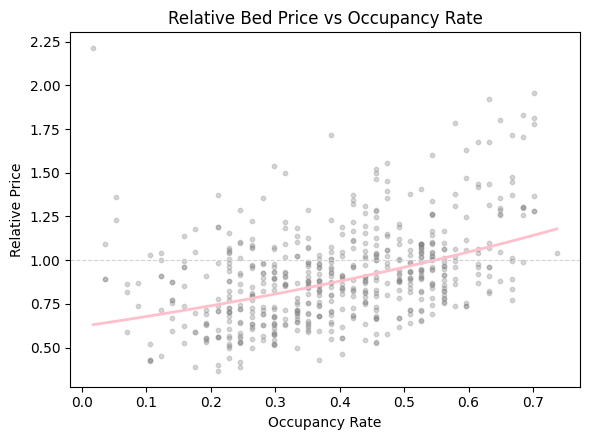
\includegraphics[width=\linewidth]{price_demand_corr.png}
    \end{column}
  \end{columns}
\end{frame}

\begin{frame}{The Idea}
  \vspace{0.4em}
  \begin{center}
    
\begin{tikzpicture}[
        node distance=1.0cm,
        arr/.style={->,>=stealth,line width=1.6pt,draw=muted}
      ]
      \node (hist) {\stagebox{navy}{DATA}{Historical}{booking data}};
      \node[right=1.05cm of hist] (sarima) {\stagebox{sky}{FORECAST}{Occupancy}{SARIMA}};
      \node[right=1.05cm of sarima] (kde) {\stagebox{violet}{PRICE}{Recommendation}{KDE + quantile}};

      \draw[arr] (hist.east) -- (sarima.west);
      \draw[arr] (sarima.east) -- (kde.west);
    \end{tikzpicture}
  \end{center}
\end{frame}

\begin{frame}{Model 1 -- Data}
  \begin{columns}[c,onlytextwidth]
    \begin{column}{0.48\textwidth}
      \vspace{-0.1em}
      {\color{muted}\small Daily occupancy and relative price}\par\vspace{0.45em}
      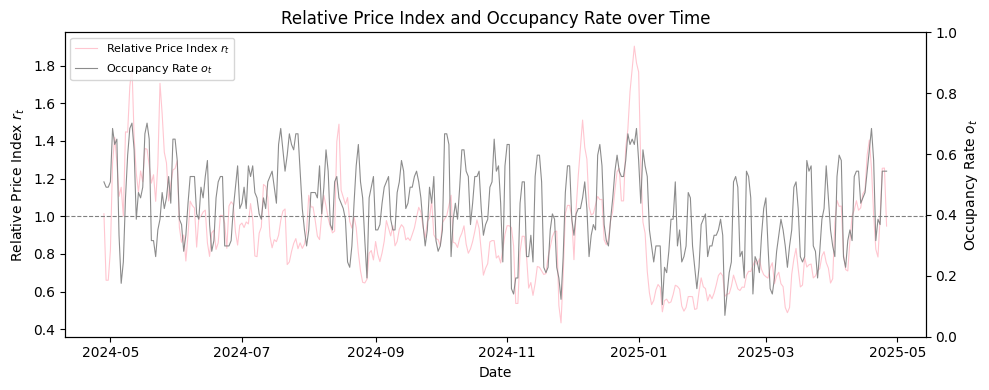
\includegraphics[width=\linewidth,height=0.58\paperheight,keepaspectratio]{timeseries_basic.png}
    \end{column}
    \begin{column}{0.48\textwidth}
      \vspace{-0.1em}
      {\color{muted}\small Occupancy--price relation, $\rho=0.583$}\par\vspace{0.45em}
      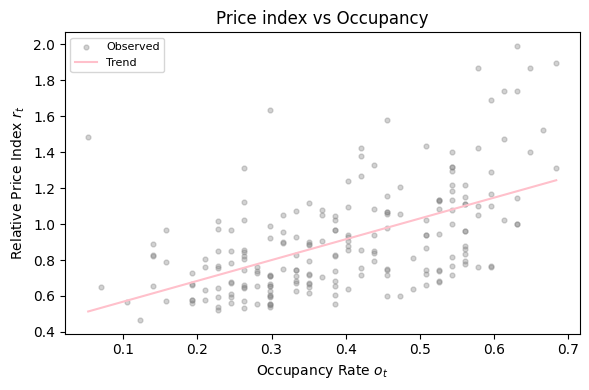
\includegraphics[width=\linewidth,height=0.58\paperheight,keepaspectratio]{price_occupancy.png}
    \end{column}
  \end{columns}
\end{frame}

\begin{frame}{Model 2 -- Occupancy Forecast}
  \begin{tikzpicture}[remember picture,overlay]
    \shade[top color=violet,bottom color=aqua,opacity=0.96]
    ([xshift=0.60\paperwidth]current page.north west) rectangle (current page.south east);
    \fill[white,opacity=0.11]
    ([xshift=0.65\paperwidth,yshift=-0.10\paperheight]current page.north west)
    rectangle ([xshift=0.80\paperwidth,yshift=-0.34\paperheight]current page.north west);
    \fill[white,opacity=0.08]
    ([xshift=0.75\paperwidth,yshift=-0.50\paperheight]current page.north west)
    rectangle ([xshift=\paperwidth,yshift=-0.72\paperheight]current page.north west);
  \end{tikzpicture}%
  \begin{columns}[c,onlytextwidth]
    \begin{column}{0.55\textwidth}
      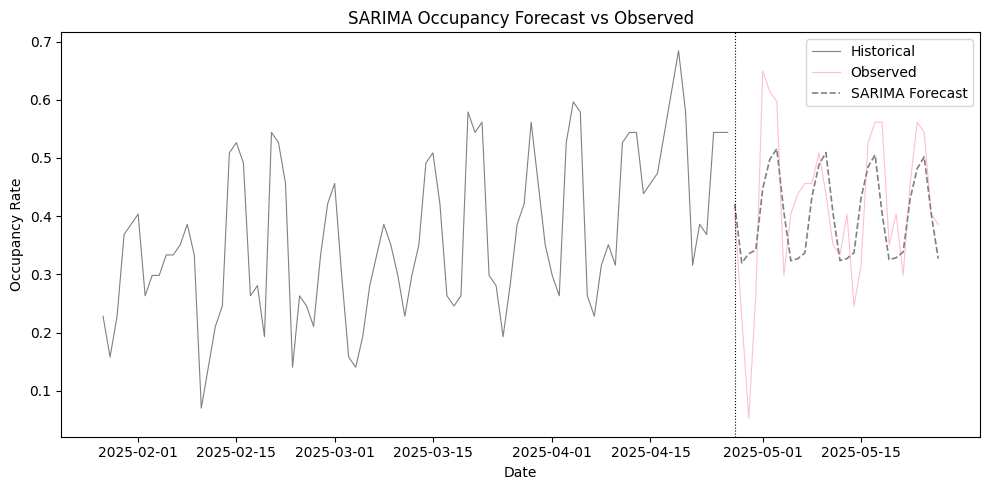
\includegraphics[width=\linewidth]{demand_prediction.png}
    \end{column}
    \begin{column}{0.34\textwidth}
      \vspace{0.4em}
      \pointrow[0.62\linewidth]{01}{{\large Occupancy input}\\{\color{muted}\small Historical series $o_t$}}\par\vspace{0.65em}
      \pointrow[0.62\linewidth]{02}{{\large SARIMA model}\\{\color{muted}\small Seasonal Autoregressive Integrated Moving Average}}\par\vspace{0.65em}
      \pointrow[0.62\linewidth]{03}{{\large Forecast output}\\{\color{muted}\small Future occupancy $\hat{o}_t$}}
    \end{column}
  \end{columns}
\end{frame}

\begin{frame}{Model 3 -- Price}
  
\begin{tikzpicture}[remember picture,overlay]
    \shade[left color=aqua,right color=violet,opacity=0.96]
    ([yshift=-0.112\paperheight]current page.north west)
    rectangle ([yshift=0.038\paperheight]current page.south east);
  \end{tikzpicture}%
  \begin{columns}[c,onlytextwidth]
    \begin{column}{0.306\textwidth}
      {\setlength{\fboxsep}{6pt}\colorbox{white}{\parbox{\dimexpr\linewidth-12pt\relax}{%
            {\small Joint density}\par\vspace{0.3em}%
            ${\color{muted}\hat{f}_{O,R}(o,r)}$%
          }}}\par\vspace{0.5em}
      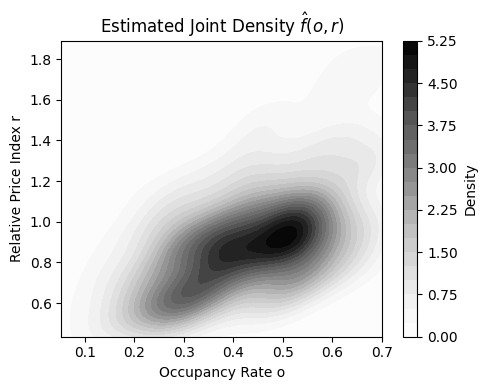
\includegraphics[width=\linewidth,height=0.38\paperheight,keepaspectratio]{KDE.png}
    \end{column}
    \begin{column}{0.48\textwidth}
      {\setlength{\fboxsep}{6pt}\colorbox{white}{\parbox{\dimexpr\linewidth-12pt\relax}{%
      {\small Conditional quantile recommendation}\par\vspace{0.3em}%
      ${\color{muted}p_{a,t}^*=\hat{F}_{R|O}^{-1}(\alpha\mid\hat{o}_t)\,\bar p_a}$%
      }}}\par\vspace{0.5em}
      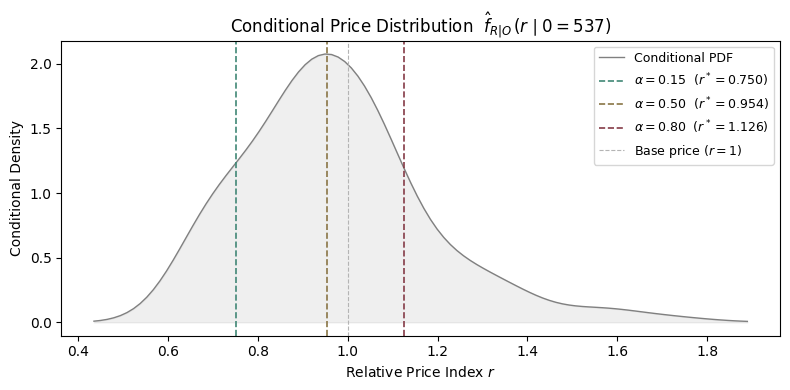
\includegraphics[width=\linewidth,height=0.60\paperheight,keepaspectratio]{pricing_quantiles.png}
    \end{column}
  \end{columns}
\end{frame}

\begin{frame}{Results -- Demand Forecast}
  \begin{columns}[T,onlytextwidth]
    \begin{column}{0.62\textwidth}
      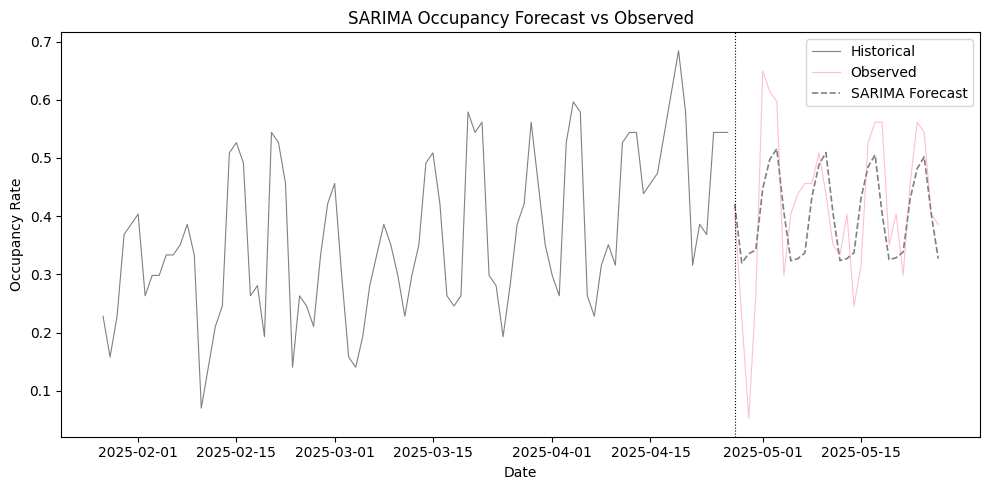
\includegraphics[width=\linewidth]{demand_prediction.png}
    \end{column}
    \begin{column}{0.34\textwidth}
      \vspace{0.8em}
      \metricbox{0.78\linewidth}{SARIMA MAE}{0.073}\par\vspace{0.75em}
      \metricbox{0.78\linewidth}{Improvement vs. naive}{-22\,\%}\par\vspace{0.95em}
    \end{column}
  \end{columns}
\end{frame}

\begin{frame}{Results -- Price Recommendations}
  \begin{tikzpicture}[remember picture,overlay]
    \shade[top color=aqua,bottom color=violet,opacity=0.96]
    ([xshift=0.60\paperwidth]current page.north west) rectangle (current page.south east);
    \fill[white,opacity=0.11]
    ([xshift=0.65\paperwidth,yshift=-0.10\paperheight]current page.north west)
    rectangle ([xshift=0.80\paperwidth,yshift=-0.34\paperheight]current page.north west);
    \fill[white,opacity=0.08]
    ([xshift=0.75\paperwidth,yshift=-0.50\paperheight]current page.north west)
    rectangle ([xshift=\paperwidth,yshift=-0.72\paperheight]current page.north west);
    \node[anchor=north] at ([xshift=0.80\paperwidth,yshift=-0.04\paperheight]current page.north west) {
      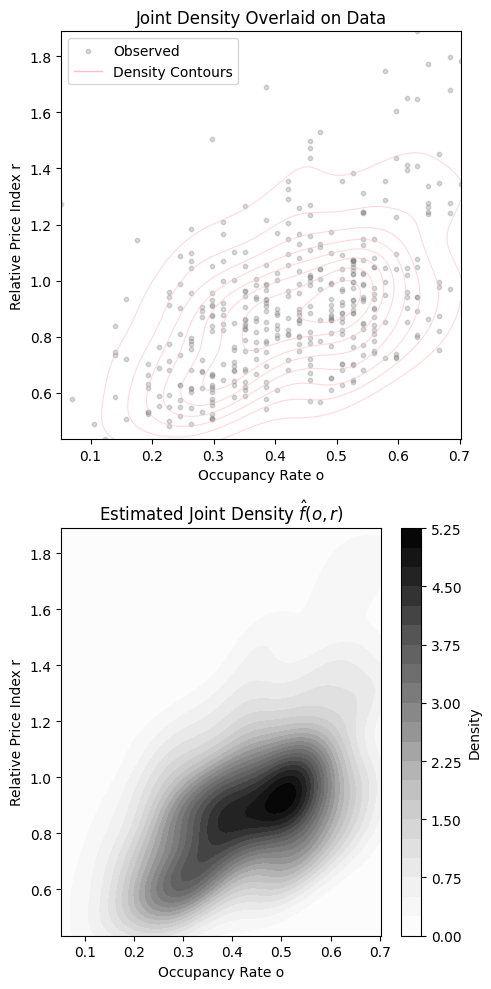
\includegraphics[width=0.4\paperwidth,height=0.88\paperheight,keepaspectratio]{estimated_density_vert.png}
    };
  \end{tikzpicture}
  \begin{columns}[T,onlytextwidth]
    \begin{column}{0.58\textwidth}
      \metricbox{0.82\linewidth}{Evaluation sample}{290 apartment-days}\par\vspace{0.65em}
      \metricbox{0.82\linewidth}{Systematic bias}{-4.2\,\%}\par\vspace{0.65em}
      \metricbox{0.82\linewidth}{Mean abs. error}{28.4\,\%}\par\vspace{1.8em}
    \end{column}
  \end{columns}
\end{frame}

\begin{frame}{Limitations}
  \rightpanel
  \vspace{0.45em}
  \begin{minipage}{0.70\linewidth}
    \pointrow{01}{{\large SARIMA smoothing effect}\\{\color{muted}\small Sharp local shocks are deliberately dampened.}}\par\vspace{0.68em}
    \pointrow{02}{{\large No external variables}\\{\color{muted}\small Events, weather, and competitors are outside the current model.}}\par\vspace{0.68em}
    \pointrow{03}{{\large Fixed $\alpha$}\\{\color{muted}\small Risk appetite is not adapted by apartment or date.}}\par\vspace{0.68em}
    \pointrow{04}{{\large Limited provider data}\\{\color{muted}\small Validation uses one provider and a short observation window.}}
  \end{minipage}
\end{frame}

\end{document}
